%% Springer Nature single-column manuscript (sn-jnl, "sn-basic" reference style), condensed to about ten pages.
%% Numbers come from ../numbers.tex (generated from the frozen results file). The full-length text is main_full.tex.
\documentclass[pdflatex,sn-basic]{sn-jnl}

\usepackage{graphicx}
\usepackage{multirow}
\usepackage{amsmath,amssymb,amsfonts}
\usepackage{amsthm}
\usepackage{mathrsfs}
\usepackage{xcolor}
\usepackage{textcomp}
\usepackage{manyfoot}
\usepackage{booktabs}
\usepackage[hyphens]{xurl}

\graphicspath{{../../docs/figures/}}
% GENERATED by `python -m src.report.paper_numbers`. Do not edit: change the freeze and regenerate.
% source: benchmarks/results_freeze_v5.json  sha256 4ada25e3b5a99a4b  frozen_at 2026-10-21T11:19:28.292835+00:00  values 109
\providecommand{\fzLegsTotal}{26{,}369} % legs_total (legs)
\providecommand{\fzCorridorsTotal}{2{,}783} % corridors_total (corridors)
\providecommand{\fzMedianGapRatio}{2} % median_gap_ratio (x)
\providecommand{\fzCorridorsTested}{1{,}130} % corridors_tested (corridors)
\providecommand{\fzBottlenecks}{273} % bottlenecks (corridors)
\providecommand{\fzFasterCorridors}{512} % faster_corridors (corridors)
\providecommand{\fzLegsCovered}{20{,}739} % legs_covered (legs)
\providecommand{\fzRobustnessBottlenecks}{34} % robustness_bottlenecks (corridors)
\providecommand{\fzSplitTrain}{21{,}095} % split_train (legs)
\providecommand{\fzSplitTest}{5{,}274} % split_test (legs)
\providecommand{\fzPctDelayed}{49.69} % pct_delayed (%)
\providecommand{\fzMaeOsrm}{107.09} % mae_osrm (min)
\providecommand{\fzMaeCorridorMean}{36.13} % mae_corridor_mean (min)
\providecommand{\fzChampionModel}{random\_forest} % champion_model (text)
\providecommand{\fzMaeChampion}{36.89} % mae_champion (min)
\providecommand{\fzCorridorsImproved}{1{,}369} % corridors_improved (corridors)
\providecommand{\fzDocAgentFOneVOne}{0.853} % doc_agent_f1_v1 (text)
\providecommand{\fzDocAgentFOneVTwo}{0.929} % doc_agent_f1_v2 (text)
\providecommand{\fzStreamIdentical}{500} % stream_identical (of 500)
\providecommand{\fzStreamEvents}{52{,}738} % stream_events (events)
\providecommand{\fzStreamProducedEps}{886.4} % stream_produced_eps (events/sec)
\providecommand{\fzStreamScoringEps}{739.9} % stream_scoring_eps (events/sec)
\providecommand{\fzStreamLatencyPFiveZeroS}{28.9} % stream_latency_p50_s (s)
\providecommand{\fzOrderEvalRun}{50} % order_eval_run (of 50)
\providecommand{\fzOrderEvalSuccess}{1} % order_eval_success (text)
\providecommand{\fzOrderEvalInvented}{0} % order_eval_invented (orders)
\providecommand{\fzLifecycleCases}{10} % lifecycle_cases (cases)
\providecommand{\fzLifecycleBooked}{5} % lifecycle_booked (cases)
\providecommand{\fzLifecycleTicketed}{2} % lifecycle_ticketed (cases)
\providecommand{\fzInvoiceCases}{20} % invoice_cases (invoices)
\providecommand{\fzInvoiceCorrect}{20} % invoice_correct (invoices)
\providecommand{\fzMedianBarMae}{33.04} % median_bar_mae (min)
\providecommand{\fzModelVTwoMae}{30.9} % model_v2_mae (min)
\providecommand{\fzDocExtractionAccuracy}{0.9786} % doc_extraction_accuracy (share)
\providecommand{\fzDocExtractionRows}{20} % doc_extraction_rows (rows)
\providecommand{\fzAssistantRouteAccuracy}{0.9} % assistant_route_accuracy (share)
\providecommand{\fzScaleRows}{56{,}353{,}613} % scale_rows (rows)
\providecommand{\fzExceptionPrecisionAsOf}{0.5855} % exception_precision_as_of (share)
\providecommand{\fzAssistantGroundedness}{0.9444} % assistant_groundedness (share)
\providecommand{\fzKafkaFileAlertsIdentical}{true} % kafka_file_alerts_identical (bool)
\providecommand{\fzAdoptedStreamEqualsBatch}{500} % adopted_stream_equals_batch (legs)
\providecommand{\fzFreshCloneRebuildS}{4{,}258} % fresh_clone_rebuild_s (seconds)
\providecommand{\fzOrderEvalScaleHeldout}{0.85} % order_eval_scale_heldout (share)
\providecommand{\fzOrderEvalScaleAdversarialHeldout}{0.7} % order_eval_scale_adversarial_heldout (share)
\providecommand{\fzOrderEvalScaleCases}{200} % order_eval_scale_cases (cases)
\providecommand{\fzInvoiceEvalScaleAccuracy}{0.9} % invoice_eval_scale_accuracy (share)
\providecommand{\fzInvoiceEvalScaleCases}{200} % invoice_eval_scale_cases (invoices)
\providecommand{\fzInvoiceEvalScaleFalseDisputes}{0} % invoice_eval_scale_false_disputes (invoices)
\providecommand{\fzLifecycleEvalScalePaths}{3} % lifecycle_eval_scale_paths (of 3)
\providecommand{\fzLifecycleEvalScaleRouting}{1} % lifecycle_eval_scale_routing (share)
\providecommand{\fzLifecycleEvalScaleCases}{100} % lifecycle_eval_scale_cases (lifecycles)
\providecommand{\fzBarOldMedianMae}{33.0423} % bar_old_median_mae (min)
\providecommand{\fzBarBackoffMae}{32.3932} % bar_backoff_mae (min)
\providecommand{\fzBarShrunkMae}{32.9221} % bar_shrunk_mae (min)
\providecommand{\fzBarBackoffValidationMae}{29.3567} % bar_backoff_validation_mae (min)
\providecommand{\fzColdLegsTest}{204} % cold_legs_test (legs)
\providecommand{\fzColdMaeBackoff}{132.9706} % cold_mae_backoff (min)
\providecommand{\fzColdMaeModel}{100.1619} % cold_mae_model (min)
\providecommand{\fzWarmMaeBackoff}{28.3464} % warm_mae_backoff (min)
\providecommand{\fzWarmMaeModel}{28.1182} % warm_mae_model (min)
\providecommand{\fzVThreeValidationMae}{31.1425} % v3_validation_mae (min)
\providecommand{\fzVTwoValidationMae}{30.17} % v2_validation_mae (min)
\providecommand{\fzVThreeTestMae}{31.4032} % v3_test_mae (min)
\providecommand{\fzServedVsBarDelta}{-1.4884} % served_vs_bar_delta (min)
\providecommand{\fzServedVsBarCiLow}{-2.2465} % served_vs_bar_ci_low (min)
\providecommand{\fzServedVsBarCiHigh}{-0.738} % served_vs_bar_ci_high (min)
\providecommand{\fzServedMaeCiLow}{29.0171} % served_mae_ci_low (min)
\providecommand{\fzServedMaeCiHigh}{32.6355} % served_mae_ci_high (min)
\providecommand{\fzAuditRobustHeadlineSlower}{0} % audit_robust_headline_slower (corridors)
\providecommand{\fzAuditRobustHeadlineFaster}{0} % audit_robust_headline_faster (corridors)
\providecommand{\fzAuditByWelchSlower}{218} % audit_by_welch_slower (corridors)
\providecommand{\fzAuditPlaceboRejection}{0.6387} % audit_placebo_rejection (share)
\providecommand{\fzAuditPlaceboDiscoveries}{680.205} % audit_placebo_discoveries (corridors)
\providecommand{\fzEbThresholdLog}{1.1838} % eb_threshold_log (log)
\providecommand{\fzEbTopTwoZeroJaccardRaw}{0.1012} % eb_top20_jaccard_raw (jaccard)
\providecommand{\fzEbTopTwoZeroJaccardEb}{0.1502} % eb_top20_jaccard_eb (jaccard)
\providecommand{\fzStabilityUniverse}{807} % stability_universe (corridors)
\providecommand{\fzStabilityJaccard}{0.6364} % stability_jaccard (jaccard)
\providecommand{\fzStabilitySpearman}{0.9084} % stability_spearman (rho)
\providecommand{\fzStabilityStillSlower}{0.9769} % stability_still_slower (share)
\providecommand{\fzStabilityBaseRate}{0.3978} % stability_base_rate (share)
\providecommand{\fzReportedMae}{29.6578} % reported_mae (min)
\providecommand{\fzReportedMaeCiLow}{27.8611} % reported_mae_ci_low (min)
\providecommand{\fzReportedMaeCiHigh}{31.1193} % reported_mae_ci_high (min)
\providecommand{\fzReportedVsBarDelta}{-2.7354} % reported_vs_bar_delta (min)
\providecommand{\fzReportedVsBarCiLow}{-3.4132} % reported_vs_bar_ci_low (min)
\providecommand{\fzReportedVsBarCiHigh}{-2.107} % reported_vs_bar_ci_high (min)
\providecommand{\fzReportedValidationMae}{27.2368} % reported_validation_mae (min)
\providecommand{\fzZooLightgbmHuberMae}{30.5347} % zoo_lightgbm_huber_mae (min)
\providecommand{\fzZooXgboostMae}{29.7104} % zoo_xgboost_mae (min)
\providecommand{\fzZooHistgbrMae}{29.7456} % zoo_histgbr_mae (min)
\providecommand{\fzZooLinearMae}{33.9563} % zoo_linear_mae (min)
\providecommand{\fzExcPrecisionAsOfRate}{0.5855} % exc_precision_as_of_rate (share)
\providecommand{\fzExcPrecisionCiLow}{0.562} % exc_precision_ci_low (share)
\providecommand{\fzExcPrecisionCiHigh}{0.6085} % exc_precision_ci_high (share)
\providecommand{\fzExcAlerts}{1{,}720} % exc_alerts (legs)
\providecommand{\fzExcGainPoints}{4.45} % exc_gain_points (points)
\providecommand{\fzExcGainCiLow}{0.0353} % exc_gain_ci_low (share)
\providecommand{\fzExcGainCiHigh}{0.0538} % exc_gain_ci_high (share)
\providecommand{\fzExcGainZ}{9.8904} % exc_gain_z (z)
\providecommand{\fzAblationOrderCases}{18} % ablation_order_cases (cases)
\providecommand{\fzAblationOrderLlmAccuracy}{0.8778} % ablation_order_llm_accuracy (share)
\providecommand{\fzAblationOrderLlmCiLow}{0.7943} % ablation_order_llm_ci_low (share)
\providecommand{\fzAblationOrderLlmCiHigh}{0.9304} % ablation_order_llm_ci_high (share)
\providecommand{\fzAblationOrderUnanimity}{0.8333} % ablation_order_unanimity (share)
\providecommand{\fzAblationOrderKappa}{0.82} % ablation_order_kappa (kappa)
\providecommand{\fzHardOrderRules}{0.7} % hard_order_rules (share)
\providecommand{\fzHardOrderCases}{100} % hard_order_cases (cases)
\providecommand{\fzHardInvoiceRules}{1} % hard_invoice_rules (share)


\newcommand{\mentorgiven}{Anshi}
\newcommand{\mentorsurname}{Bajaj}
\newcommand{\mentoremail}{anshi.bajaj@nmims.edu}

\begin{document}

\title[Localising Route-Estimate Error in Road Freight]{Localising Systematic Route-Estimate Error in Road Freight: Dependence-Aware Corridor Auditing, Residual Prediction and a Measured Agent Layer}

\author*[1]{\fnm{Kuchuru Sai Krishna} \sur{Reddy}}\email{kuchurusaikrishnareddy@gmail.com}
\equalcont{These authors contributed equally to this work.}

\author[1]{\fnm{Makkena} \sur{Lahari}}\email{laharisuresh6666@gmail.com}
\equalcont{These authors contributed equally to this work.}

\author[1]{\fnm{Shery Mounika} \sur{Reddy}}\email{sherymounikareddy.2006@gmail.com}
\equalcont{These authors contributed equally to this work.}

\author[1]{\fnm{\mentorgiven} \sur{\mentorsurname}}\email{\mentoremail}

\affil*[1]{\orgdiv{Department of Computer Science and Data Science}, \orgname{SVKM's Narsee Monjee Institute of Management Studies}, \city{Hyderabad}, \country{India}}

\abstract{Road-freight operators schedule against route-planner estimates, and the OSRM estimate recorded in Delhivery's public trip data runs short almost every time: \fzLegsTotal{} legs, the median taking \fzMedianGapRatioDpOne{} times the estimate. We ask where this error concentrates and how confidently that can be said. A Welch audit with false-discovery control flags \fzBottlenecks{} corridors as slower than the network, but legs of one recurring service are correlated (design effect about \fzDepDesignEffectMedianDpOne{}), and on placebo data with meaningless corridor labels the same procedure returns about \fzAuditPlaceboDiscoveriesDpOne{} discoveries; a cluster-aware permutation test confirms \fzAuditRobustHeadlineSlower{} corridors at its pre-registered strictness. Corridor effects nonetheless persist between halves of the period (rank correlation \fzStabilitySpearmanDpTwo{}), and empirical-Bayes ranking is only slightly more stable across support floors than raw ranking. For prediction, a gradient-boosted residual over a hierarchical back-off baseline, whose cold-start fallback is fair, reaches \fzReportedMaeDpTwo{} minutes MAE against the baseline's \fzBarBackoffMaeDpTwo{} (difference \fzReportedVsBarDeltaDpTwo{}, day-block 95\% interval [\fzReportedVsBarCiLowDpTwo{}, \fzReportedVsBarCiHighDpTwo{}]), with the gain on corridors without history. We report two evaluation pitfalls, an optimiser default that disabled the chosen loss and a replay that inflated an alert precision to 72.1\% that is \fzExcPrecisionAsOfRatePct{}\% once history is joined as of each event. Code, pre-registrations and every result file are public.
}

\keywords{route planning, travel-time reliability, multiple testing, gradient boosting, stream processing, language-model agents}

\maketitle

\section{Introduction}\label{sec:intro}
A route planner's estimate is a plan, and a plan that is consistently optimistic is still useful if the operator knows \emph{where} it is optimistic. The public trip records of Delhivery, an Indian road-freight carrier\footnote{Kaggle dataset ``Delhivery logistics dataset'' (user \texttt{devarajv88}); licence terms are in \texttt{DATA\_LICENSE.md} of the repository.}, carry for every leg both a planned time recorded from OSRM~\cite{luxen2011real} and the realised time, so the question can be put to operational data directly. Across \fzLegsTotal{} legs, 98.3\% exceed the recorded estimate and the median leg takes \fzMedianGapRatioDpOne{} times it (Fig.~\ref{fig:premise}). Noise would centre on one, so the error is systematic; but a systematic error is not automatically \emph{localised}, since it could be spread evenly and removed by one correction factor. We ask where it concentrates, how confidently that can be said, and what a model can do about it, and we report the answers at the strength the data support rather than the strength a first analysis gave.

\begin{figure}[!htb]
\centering
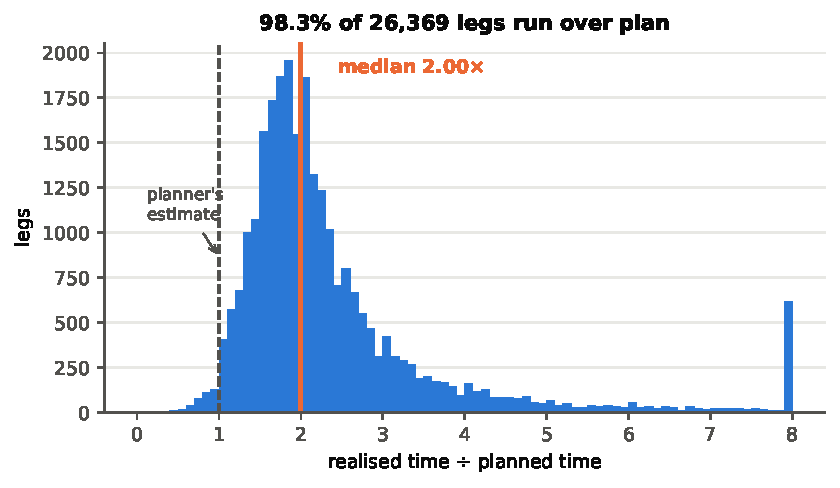
\includegraphics[width=0.5\textwidth]{fig1_gap_ratio_distribution.pdf}
\caption{Realised over recorded planned time across \fzLegsTotal{} legs. The mass sits well to the right of 1.0: 98.3\% of legs run over the estimate.}
\label{fig:premise}
\end{figure}

A first analysis was more flattering than the one reported here. A Welch test with false-discovery control found \fzBottlenecks{} corridors significantly slower than the network; a test that respects the dependence between legs of one recurring service finds that the same procedure on meaningless corridor labels returns about \fzAuditPlaceboDiscoveriesDpOne{} ``bottlenecks''. A residual model first beat its baseline by 6.5\%; against a baseline without an unfair cold-start fallback the margin is smaller. Our contributions are:
\begin{enumerate}
\item \textbf{A way to measure a corridor audit's own error.} A placebo (real cell structure, no corridor effect) and a power simulation show that the standard audit is wrong in about \fzPowerWelchBhFdpShiftHalfPct{}\% of its discoveries here, and that the dependence-aware replacement is correctly sized but finds only \fzPowerByPermShiftOnePct{}\% of corridors even when a 2.7-fold overrun is planted. A zero from such a test cannot be read as absence.
\item \textbf{A dependence-aware audit and evidence that corridor effects persist}: a permutation test whose unit is the (corridor, service) cell confirms \fzAuditRobustHeadlineSlower{} of the \fzBottlenecks{} slow corridors, yet corridor means correlate at \fzStabilitySpearmanDpTwo{} between the two halves of the period.
\item \textbf{Two remedies that do not rescue the ranking}: empirical-Bayes shrinkage and the standard planning-time and buffer indices.
\item \textbf{A residual model over a fair baseline}, with day-block intervals, rolling folds and an exact serving proof through a streaming job.
\item \textbf{Two evaluation pitfalls}, and a measured, pilot-scale look at language-model agents.
\end{enumerate}
We do not claim to beat the planner: OSRM has no access to corridor history, and a model that does is not a fair comparison.

\section{Related Work}\label{sec:related}
OSRM is an open-source routing engine~\cite{luxen2011real}; DeeprETA~\cite{hu2022deepreta} post-processes a planner's estimate with a learned residual, the structure we use, while we make localising the planner's error primary. Transport research describes corridors with planning-time and buffer indices~\cite{fhwa2005reliability,jones2005measuring}; we add multiplicity-controlled testing that respects dependence. False-discovery control~\cite{benjamini1995controlling,benjamini2001control}, permutation tests~\cite{phipson2010permutation} and cluster-robust inference~\cite{cameron2015practitioner} frame the audit, empirical-Bayes ranking~\cite{efron1975data,morris1983parametric} the shrinkage, and rolling-origin evaluation~\cite{tashman2000out} and the leakage literature~\cite{kaufman2012leakage,kapoor2023leakage} the evaluation. Agents that interleave reasoning with tool calls~\cite{yao2023react} follow the division of labour of OptiGuide~\cite{li2023optiguide}, where a model explains an optimiser's output while the optimiser decides. We found notebooks on this dataset but no peer-reviewed study; that is a statement about our search, not the world.

\section{Data and Problem Definition}\label{sec:data}
The raw records are 144,867 scan-level segments across 14,817 trips between 12 September and 8 October 2018. They are reconstructed into \fzLegsTotal{} origin--destination \emph{legs} on \fzCorridorsTotal{} \emph{corridors} (ordered facility pairs) touching 1,657 facilities; \fzCorridorsTested{} corridors have at least 10 legs and are tested, and the chronological split has \fzSplitTrain{} training and \fzSplitTest{} test legs, of which \fzColdLegsTest{} have no prior leg on their corridor (cold). The planned time is the dataset's \texttt{osrm\_time} column; we cannot know the OSRM version, the profile, or whether the carrier used it operationally, so we make no claim about the carrier's planning system. For leg $i$ let $a_i$ be realised moving time and $o_i$ the recorded OSRM time in minutes; the \emph{log ratio} is $r_i=\log(a_i/o_i)$ and the \emph{gap} is $g_i=a_i-o_i$. The audit uses $r_i$; prediction uses $g_i$, because the metric is minutes. Dwell at the hub is separated from movement.



\paragraph{As-of features.} Every feature describing a corridor's or hub's history is computed only from legs that had \emph{finished} before the leg in question was \emph{created}. Legs with no prior leg on their corridor carry an explicit cold indicator rather than a zero. We verified the rule with an independent reconstruction of the as-of history; it agrees with the production implementation on every leg with history (before one correction it agreed on 95.2\%, which is how the error was found).

\section{The Corridor Audit}\label{sec:audit}
\subsection{Method}
For corridor $c$ with $n_c\ge10$ legs the statistic is Welch's $t$ for the corridor's mean log ratio against the mean over all other legs, corrected for $m=\fzCorridorsTested{}$ tests by Benjamini--Hochberg (BH) at 0.05~\cite{benjamini1995controlling} or by Benjamini--Yekutieli (BY), which is valid under arbitrary dependence~\cite{benjamini2001control}.

Welch's test treats legs as independent, so we measured the dependence first. Trips do not cluster a corridor's legs (intraclass correlation 0.07, and no trip visits a corridor twice) and the creation day is almost irrelevant (under 0.01). What clusters is the recurring \emph{service}: legs of one (corridor, service) cell have intraclass correlation \fzDepIccServiceCellDpTwo{}, a design effect of \fzDepDesignEffectMedianDpTwo{} at the median corridor, whose 15 legs carry the information of about 7 independent ones. For the \fzDepSingleServiceCorridors{} corridors that run under one service, a corridor effect and a service effect cannot be told apart.

The exchangeable unit is therefore the cell. Cells are stratified by size and one permutation shuffles cell means among cells of the same stratum; the $p$-value is two-sided with $B=100{,}000$ permutations~\cite{phipson2010permutation}. A rule fixed in advance names the \emph{headline} as the valid variant with the fewest significant slower corridors. We measure the standard test's size with a placebo of 200 datasets in which cell means are permuted among cells, destroying any corridor effect while keeping the cluster structure.

\subsection{Result}
\begin{table}[!htb]
\caption{Corridors significant at 5\% under four variants of the audit, of \fzCorridorsTested{} tested.}
\label{tab:variants}
\centering
\begin{tabular}{@{}lrr@{}}
\toprule
Variant & Slower & Faster \\
\midrule
Welch, BH (the original audit) & \fzBottlenecks{} & \fzFasterCorridors{} \\
Welch, BY & \fzAuditByWelchSlower{} & \fzAuditByWelchFaster{} \\
Cell permutation, BH & \fzAuditBhPermSlower{} & \fzAuditBhPermFaster{} \\
\textbf{Cell permutation, BY (headline)} & \textbf{\fzAuditRobustHeadlineSlower{}} & \textbf{\fzAuditRobustHeadlineFaster{}} \\
\bottomrule
\end{tabular}
\end{table}
The original procedure finds \fzBottlenecks{} slower and \fzFasterCorridors{} faster corridors, covering 78.6\% of legs. Under the cell permutation the counts collapse (Table~\ref{tab:variants}), and by the pre-registered rule the headline is \textbf{\fzAuditRobustHeadlineSlower{} slower and \fzAuditRobustHeadlineFaster{} faster}. The placebo explains why: with no corridor information, Welch rejects \fzAuditPlaceboRejectionPct{}\% of corridors uncorrected at the nominal 5\%, and Welch with BH finds on average \fzAuditPlaceboDiscoveriesDpOne{} ``significant'' corridors, against 785 on the real data. The \fzBottlenecks{} are therefore a \emph{screening list}, not confirmed bottlenecks.

\paragraph{What a zero means.} A zero is ambiguous between no effect and a test too weak to see one, so we planted known shifts of the log ratio into 30 corridors of the placebo world and ran all four variants on 30 simulated datasets per shift (Fig.~\ref{fig:power}). The cell-permutation test is correctly sized (\fzPowerPermSizeByPct{}\% of null datasets show a BY rejection) and nearly blind: at a shift of 1.0, a 2.7-fold overrun, it finds \fzPowerByPermShiftOnePct{}\% of planted corridors under BY and \fzPowerBhPermShiftOnePct{}\% under BH, and never reaches 80\% power. Welch finds planted corridors easily, but at a shift of 0.5 \fzPowerWelchBhFdpShiftHalfPct{}\% of its discoveries are not planted ones (nominal 5\%). So the zero says almost nothing about whether corridor effects exist, and corridor effects rest instead on the persistence result below.

\begin{figure}[!htb]
\centering
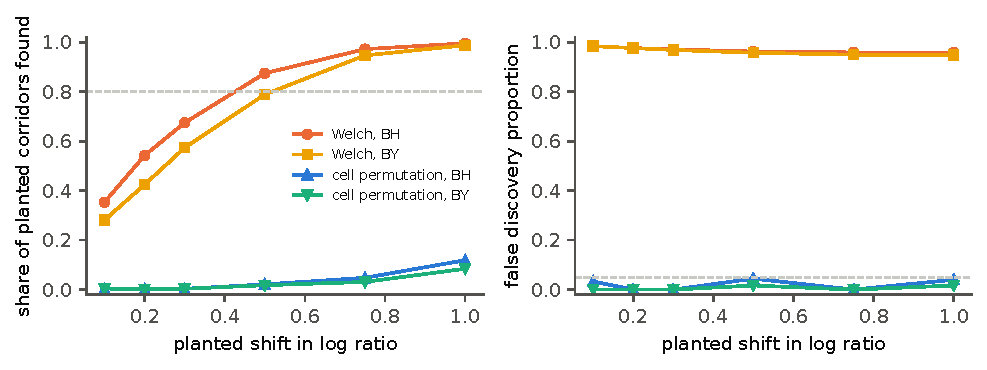
\includegraphics[width=0.85\textwidth]{fig_power_curves.pdf}
\caption{Simulated power (left) and false discovery proportion (right) of the four audit variants as a known shift is planted into 30 corridors of the placebo world; dashed lines mark 80\% power and the nominal 5\%.}
\label{fig:power}
\end{figure}

\subsection{Persistence and ranking}\label{sec:stability}
We split the creation dates into two halves and run the audit in each. Over the \fzStabilityUniverse{} corridors testable in both, raw corridor means correlate at $\rho=\fzStabilitySpearmanDpTwo{}$ (Fig.~\ref{fig:stab}), and \fzStabilityStillSlowerPct{}\% of the first half's slower corridors are also slower in the second, against a base rate of \fzStabilityBaseRatePct{}\%. The cell-permutation test finds nothing in either half; the two facts fit together because the pattern is persistent but not separable from a service effect, and the same services run in both halves, so persistence is not independent replication. Of the standard reliability indices, the mean log ratio is the most stable between halves (\fzIdxStabMeanDpTwo{}), the planning-time index less so (\fzIdxStabPtiDpTwo{}) and the buffer index least (\fzIdxStabBiDpTwo{}), so they add nothing the mean does not carry at 10 to 15 legs.

\begin{figure}[!htb]
\centering
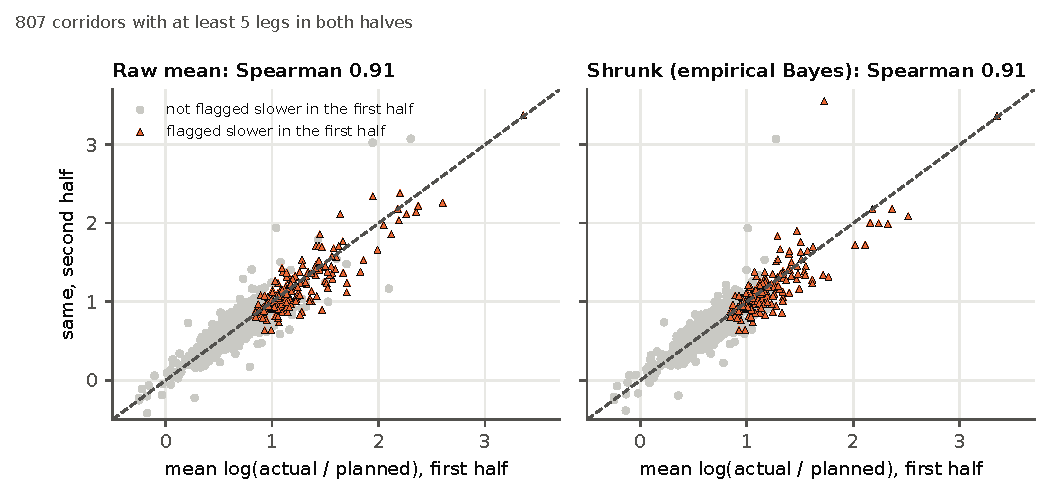
\includegraphics[width=0.42\textwidth]{b5_stability_scatter.pdf}
\caption{Corridor effects in the first half of the period against the second half.}
\label{fig:stab}
\end{figure}

Empirical-Bayes shrinkage does not rescue a top-20 list either. We model corridor means as normal around corridor effects and rank corridors by the posterior probability that the true ratio exceeds a material threshold~\cite{efron1975data,morris1983parametric}. The corridors' own sampling variances are small against the between-corridor variance, so the median shrink factor is only 1\% to 2\%. The ranking is marginally more stable across support floors (top-20 overlap \fzEbTopTwentyJaccardEbDpTwo{} against \fzEbTopTwentyJaccardRawDpTwo{} for raw means), but floors 5 and 30 share no top-20 corridor in either. The cause is eligibility, not noise: a lower floor admits small corridors with extreme means. A heavy-tailed Student-$t$ prior fits better (by \fzEbtLoglikGainFloorTenDpOne{} log-likelihood units) but gives the same overlap (\fzEbtTopTwentyJaccardDpTwo{}). We recommend reporting the whole ranking with intervals and the floor, not a top-20.

\section{Predicting the Gap}\label{sec:prediction}
\subsection{Setup and the bar}
The target is the gap in minutes, known when the leg is created, and the metric is mean absolute error (MAE), so the comparator is an as-of \emph{median}. The chronological split uses \fzSplitTrain{} training legs and the latest \fzSplitTest{} for test. A per-corridor median predicts 0.0 minutes on a corridor with no history, which is exactly the OSRM estimate the paper shows to be wrong, so we fixed before measuring a hierarchy of as-of medians: corridor, origin hub, destination hub, route type and distance band, network. This \emph{back-off bar} scores \fzBarBackoffMaeDpTwo{} minutes against \fzBarOldMedianMaeDpTwo{} for the old median, and is the bar.

\subsection{Models and results}
The target is the gap minus the baseline, so a model that learns nothing reproduces the baseline. Its 38 inputs are planned time and distance, departure time, route type, as-of history for the corridor and both hubs with cold indicators, corridor dispersion, a trailing seven-day mean and hub dwell. We fit two families under the same budget (200 trees, depth 6, absolute loss): distributed Spark MLlib gradient boosting~\cite{friedman2001greedy,meng2016mllib}, which the streaming path uses, and single-node LightGBM~\cite{ke2017lightgbm}, XGBoost~\cite{chen2016xgboost} and others. The reported model is whichever candidate has the lowest validation MAE; this rule was fixed in advance.

\begin{table}[!htb]
\caption{Test MAE on \fzSplitTest{} legs with day-block bootstrap 95\% intervals. The \emph{served} model is what the streaming job and public API run.}
\label{tab:mae}
\centering
\begin{tabular}{@{}lrr@{}}
\toprule
Model & Validation & Test \\
\midrule
OSRM plan (context) & --- & \fzMaeOsrm{} \\
Per-corridor mean & --- & \fzMaeCorridorMean{} \\
Old median (0.0 cold fallback) & 29.89 & \fzBarOldMedianMaeDpTwo{} \\
\textbf{Hard back-off (the bar)} & \fzBarBackoffValidationMaeDpTwo{} & \textbf{\fzBarBackoffMaeDpTwo{}} \\
Spark GBT, old median (served) & \fzVTwoValidationMaeDpTwo{} & \fzServedMaeDpTwo{} [\fzServedMaeCiLowDpOne{}, \fzServedMaeCiHighDpOne{}] \\
XGBoost, L1 & 28.00 & \fzZooXgboostMaeDpTwo{} \\
Histogram GBT, L1 & 27.54 & \fzZooHistgbrMaeDpTwo{} \\
\textbf{LightGBM, L1 (reported)} & \fzReportedValidationMaeDpTwo{} & \textbf{\fzReportedMaeDpTwo{}} [\fzReportedMaeCiLowDpOne{}, \fzReportedMaeCiHighDpOne{}] \\
\bottomrule
\end{tabular}
\end{table}

The reported model scores \fzReportedMaeDpTwo{} against the bar's \fzBarBackoffMaeDpTwo{} (Table~\ref{tab:mae}): a difference of \fzReportedVsBarDeltaDpTwo{} minutes with a day-block 95\% interval of [\fzReportedVsBarCiLowDpTwo{}, \fzReportedVsBarCiHighDpTwo{}] that excludes zero, winning all \fzSlicesTotal{} slices (Fig.~\ref{fig:forest}). The served Spark model is behind it, and the paper does not claim they are the same model. The interval resamples whole calendar days (six blocks), which is the most conservative of the three we computed and should not be over-read; a Diebold--Mariano test agrees.

\begin{figure}[!htb]
\centering
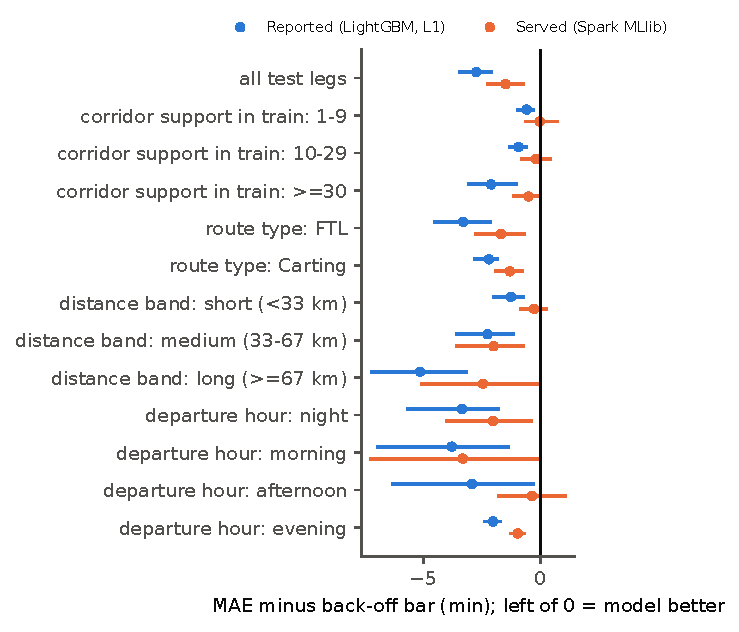
\includegraphics[width=0.5\textwidth]{fig_forest_delta_mae.pdf}
\caption{MAE minus the back-off bar by slice, for the reported (LightGBM) and served (Spark) models, with day-block 95\% intervals.}
\label{fig:forest}
\end{figure}

The whole margin sits where the bar has no history. On the \fzColdLegsTest{} cold legs the model scores \fzReportedColdMaeDpOne{} against the bar's \fzColdMaeBackoffDpOne{}; on warm legs the difference is \fzReportedWarmDeltaDpTwo{} minutes [\fzReportedWarmCiLowDpTwo{}, \fzReportedWarmCiHighDpTwo{}]. A back-off hierarchy is a strong lookup, and the model's value is mostly where a lookup has little to say. In a rolling-origin check over four expanding windows the reported model beats the bar in \fzRoZooBeatsBarFolds{} of \fzRoFolds{} folds, by \fzRoZooDeltaMeanDpTwo{} minutes on average, so the headline split is not an outlier; the deployed Spark model is not robust across folds.

\section{Streaming, Serving and the Agent Layer}\label{sec:stream}
A producer replays legs as a \emph{query} when a leg is created and a \emph{fact} when it finishes; a structured-streaming job~\cite{armbrust2018structured} scores each query and alerts when the prediction crosses twice the plan. Each fact updates the event-time state of the keys it belongs to, each query reads that state as of its own time, and the updates repeat the batch arithmetic in the same order. Over the full \fzStreamEvents{}-event replay, run in two halves across a restart, \textbf{\fzStreamAllLegsIdentical{} of \fzStreamAllLegs{} legs score bit-identically to batch}. The reported model passes the same chain exactly (\fzLgbmServeIdentical{} of \fzLgbmServeLegs{} legs through the reader, \fzLgbmStreamIdentical{} of \fzLgbmStreamLegs{} through the running stream), but the deployed path serves the Spark model because alert precision was measured on it. The job scored \fzStreamScoringEpsDpOne{} events/s with a median event-to-alert latency of \fzStreamLatencyPFiveZeroSDpOne{} s, and the public interface answers at \fzApiPNineFiveMsDpOne{} ms at the 95th percentile (Fig.~\ref{fig:arch} shows the system). On \fzScaleRows{} taxi rows the audit's aggregation ran in \fzScaleWallSDpTwo{}\,s on 20 cores, though at this project's own size the runtime is the engine's fixed cost.

\begin{figure}[!htb]
\centering
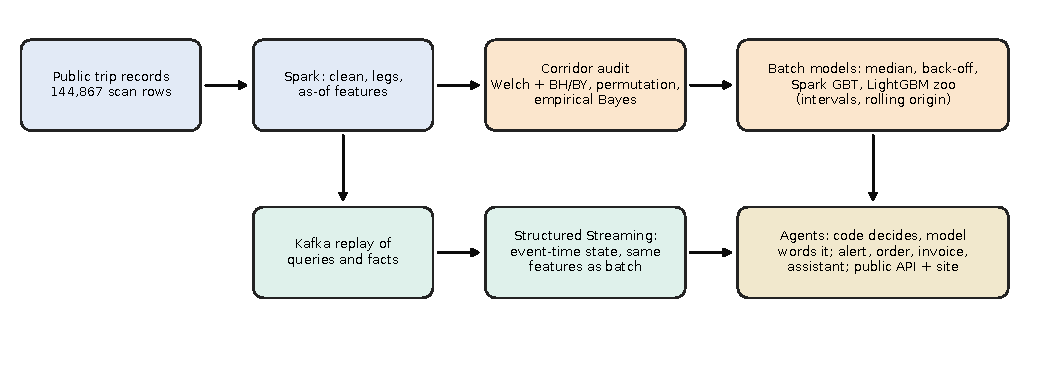
\includegraphics[width=0.8\textwidth]{fig_architecture.pdf}
\caption{System architecture: batch audit and models, streaming replay and serving, and the agent layer.}
\label{fig:arch}
\end{figure}

\paragraph{Agents.} Five agents (document extraction, order entry, exception triage, invoice audit, analytics assistant) share one rule: every verdict is computed, and a language model writes only the sentence a person reads. All agent data are synthetic; only the network data are real. At scale, order entry scored \fzOrderEvalScaleHeldoutPct{}\% on \fzOrderEvalScaleCases{} held-out emails (falling to \fzOrderEvalScaleAdversarialHeldoutPct{}\% on the adversarial half), invoice audit \fzInvoiceEvalScaleAccuracyPct{}\% on \fzInvoiceEvalScaleCases{} invoices, and the orchestrator routed \fzLifecycleEvalScaleRoutingPct{}\% of \fzLifecycleEvalScaleCases{} lifecycles correctly. In a \emph{pilot} ablation (Fig.~\ref{fig:ablation}), a 120-billion-parameter model deciding in place of the order rules scored \fzAblationOrderLlmAccuracyPct{}\% [\fzAblationOrderLlmCiLowPct{}, \fzAblationOrderLlmCiHighPct{}] with Fleiss $\kappa=\fzAblationOrderKappaDpTwo{}$ across runs and filed 12\% of orders on values the email never stated; on arithmetic policies (invoices, severity) it was comparable. The free-tier quota stopped the pre-registered sample short, and no agent decision has been compared against a second human labeller.

\begin{figure}[!htb]
\centering
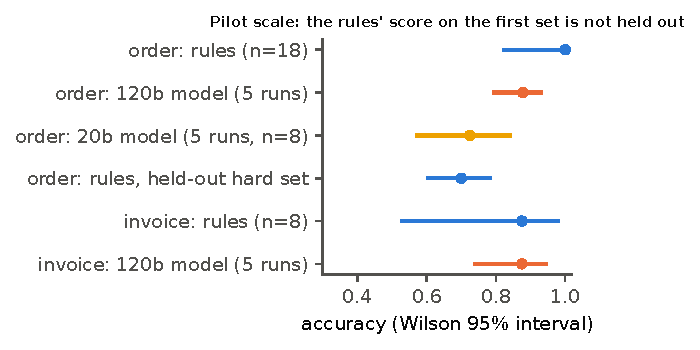
\includegraphics[width=0.6\textwidth]{fig_agent_ablation.pdf}
\caption{Pilot agent ablation: accuracy with Wilson 95\% intervals for the rule agents and a model deciding in their place. The first-set score of the rules is not held out.}
\label{fig:ablation}
\end{figure}

\section{Two Evaluation Pitfalls}\label{sec:pitfalls}
\textbf{An optimiser default that disabled the loss.} Our first distributed model used absolute-loss boosting at step size 0.05 and cleared the then bar by 1.6\%, yet lost to it on every corridor with history. The library fits the first tree with squared error and every later tree to the \emph{sign} of the error, so at 0.05 the 199 corrective trees can move a prediction by at most 9.95 minutes. When a loss is chosen to match the metric, check that the optimiser can reach it.

\textbf{A replay that scored the past with the future.} The exception agent's alert precision was first measured at 72.1\% against 54.1\% for alerting on every leg. The replay joined each query to the latest history snapshot, so 1,290 of 2,000 legs with no history at their creation time were scored as if they had fourteen prior legs. With only the history each leg had at its own time, precision is \textbf{\fzExcPrecisionAsOfRatePct{}\%} (Wilson interval [\fzExcPrecisionCiLowPct{}, \fzExcPrecisionCiHighPct{}] on \fzExcAlerts{} alerts), and the gain over alerting everything is \fzExcGainPointsDpTwo{} points, not 18. A replay is an evaluation only if every join inside it is as-of the event replayed~\cite{kaufman2012leakage,kapoor2023leakage}.

\section{Threats to Validity}\label{sec:threats}
The data are one operator, one country and 22 days of one season, so persistence is within-period and not across carriers. The planned time is the recorded OSRM number, not the carrier's own planning. The day-block interval rests on six blocks, and the validation cut favoured the bar over the Spark models while the test split favoured them, so both are shown. The permutation test is a global-null test and is resolution-limited at $10^{5}$ permutations; its zero is a limit of what these data can confirm, not proof that corridors are null. The reported and deployed models differ, and the alert evaluation was not re-run under the reported one. The agent results rest on synthetic data and a pilot sample.

\section{Conclusion}\label{sec:conclusion}
The OSRM estimate recorded in these data errs one way almost always, and that error is real but harder to localise than a first analysis suggested. The standard audit's \fzBottlenecks{} slow corridors are a screening list: the same procedure reports about \fzAuditPlaceboDiscoveriesDpOne{} discoveries when labels carry no information, and the cluster-aware test, which has little power at this sample size, confirms none at its pre-registered strictness. Corridor patterns nonetheless persist between halves. A residual model over a fair back-off bar wins by \fzReportedVsBarDeltaDpTwo{} minutes, almost all of it where the bar has no history. Our recommended protocol for corridor audits is: measure dependence and choose the exchangeable unit from it; run a placebo that keeps the structure; simulate known shifts to learn what a zero means; report the whole ranking with intervals; test persistence before calling anything a bottleneck; and judge predictive models against a baseline with a fair fallback. Future work is an audit over a longer period and several carriers, and a human-labelled evaluation of the agent layer.

\backmatter

\bmhead{Data and code availability}
The source data are public and not redistributed. All code, the decision log with every pre-registration, each result file behind a number here, and a model card and data card are at \url{https://github.com/krishna-2-005/Agentic-AI-Logistics-Control-Tower}; every number in this paper is a macro generated from a frozen results file (\texttt{benchmarks/results\_freeze\_v6.json}). An interactive version of the results is at \url{https://control-tower-mu-rouge.vercel.app}.

\bmhead{Use of AI tools}
During the preparation of this work the authors used a generative AI assistant to help draft and edit text and code. The authors reviewed and edited all content, verified every number against the underlying result files and every reference against its source, and take full responsibility for the publication.

{\footnotesize\setlength{\itemsep}{0pt}\bibliography{../refs_print}}

\end{document}
